\documentclass[11pt]{amsart}
\usepackage{geometry}                % See geometry.pdf to learn the layout options. There are lots.
\geometry{letterpaper}                   % ... or a4paper or a5paper or ... 
%\geometry{landscape}                % Activate for for rotated page geometry
%\usepackage[parfill]{parskip}    % Activate to begin paragraphs with an empty line rather than an indent
\usepackage{graphicx}
\usepackage{amssymb}
\usepackage{epstopdf}

%%%%%%%%%%%%%%%pretty code start%%%%%%%%%%%%%%%%%%%%%%%%
\usepackage[scaled]{beramono}
\usepackage{color}
\usepackage{listings}
\usepackage{setspace}
\usepackage{pdfpages}

\definecolor{Code}{rgb}{0,0,0}
\definecolor{Decorators}{rgb}{0.5,0.5,0.5}
\definecolor{Numbers}{rgb}{0.5,0,0}
\definecolor{MatchingBrackets}{rgb}{0.25,0.5,0.5}
\definecolor{Keywords}{rgb}{0,0,1}
\definecolor{self}{rgb}{0,0,0}
\definecolor{Strings}{rgb}{0,0.63,0}
\definecolor{Comments}{rgb}{0,0.63,1}
\definecolor{Backquotes}{rgb}{0,0,0}
\definecolor{Classname}{rgb}{0,0,0}
\definecolor{FunctionName}{rgb}{0,0,0}
\definecolor{Operators}{rgb}{0,0,0}
\definecolor{Background}{rgb}{0.98,0.98,0.98}

\lstnewenvironment{python}[1][]{
\lstset{
numbers=left,
numberstyle=\footnotesize,
numbersep=1em,
xleftmargin=1em,
framextopmargin=2em,
framexbottommargin=2em,
showspaces=false,
showtabs=false,
showstringspaces=false,
frame=l,
tabsize=4,
% Basic
basicstyle=\ttfamily\small\setstretch{1},
backgroundcolor=\color{Background},
language=Python,
% Comments
commentstyle=\color{Comments}\slshape,
% Strings
stringstyle=\color{Strings},
morecomment=[s][\color{Strings}]{"""}{"""},
morecomment=[s][\color{Strings}]{'''}{'''},
% keywords
morekeywords={import,from,class,def,for,while,if,is,in,elif,else,not,and,or,print,break,continue,return,True,False,None,access,as,,del,except,exec,finally,global,import,lambda,pass,print,raise,try,assert},
keywordstyle={\color{Keywords}\bfseries},
% additional keywords
morekeywords={[2]@invariant},
keywordstyle={[2]\color{Decorators}\slshape},
emph={self},
emphstyle={\color{self}\slshape},
%
}}{}

\newcommand{\prettycode}[2]{
  \hrulefill
  \subsection*{#1}
  \lstinputlisting{#2}
  \vspace{2em}
}
%%%%%%%%%%%%%%%pretty code end%%%%%%%%%%%%%%%%%%%%%%%%

\DeclareGraphicsRule{.tif}{png}{.png}{`convert #1 `dirname #1`/`basename #1 .tif`.png}

\title{STA 250: HW4: GPU Module}
\author{Christopher Conley}
\date{}                                           % Activate to display a given date or no date


\begin{document}
\maketitle
\tableofcontents
\doublespacing

\section{Question 1:  Truncated Normal Sampling}


\subsection{Implementation}

Truncated normal sampling carried out identical algorithms for both the GPU and the CPU hardware. The CPU-based code was written first in R and then in Rcpp to enhance the speed. The GPU-based code was written in C and applied in the RCUDA framework. 

 For a finite number of tries, we sampled from the normal distribution and rejected until a sample fell in the truncated interval. If that  did not succeed, then Robert one-sided truncation sampling was applied, where right or left-sided truncation was determined by whether the high truncation bound was less than the mean (right). The Robert sampling mechanism was written to handle in principle any Truncated Normal with arbitrary location, scale, or truncation interval; however, our testing revealed that some extreme tailing did reduce the accuracy of the method. \\ 

\subsection{Validating Truncation cases.}

The following plots confirm the success of our sampling implementation in a variety of truncation cases. In black, the density of 10,000 randomly sampled Normal($\mu$, $\sigma$) random variables. In red, the density of 10,000 randomly sampled Truncated Normal($\mu$, $\sigma$, $(a , b)$) random variables.The sample mean of the truncated distribution is the thick vertical red line and the blue vertical line is the expected value of the truncated normal.

\begin{figure}[htbp] %  figure placement: here, top, bottom, or page
   \centering
   \includegraphics[scale = 0.4]{../out_q1_figures/double_trunc.pdf} 
   \caption{Double truncation sampling:  TN\Big (2, 1, [0, 1.5] \Big ). Sample median (CPU $= 1.037119$, GPU $=1.035505 $ ). Expected value $= 0.9570067$} 
   \label{fig:dtrunc}
\end{figure}

\begin{figure}[htbp] %  figure placement: here, top, bottom, or page
   \centering
   \includegraphics[scale = 0.4]{../out_q1_figures/right_trunc.pdf} 
   \caption{Right truncation sampling:  TN\Big (2, 1, ($-\infty$, -3] \Big ). Sample median (CPU $= -3.129094$, GPU $= -3.13183  $ ). Expected value $= -3.186504$ } 
   \label{fig:right}
\end{figure}


\begin{figure}[htbp] %  figure placement: here, top, bottom, or page
   \centering
   \includegraphics[scale = 0.4]{../out_q1_figures/extreme_right_trunc.pdf} 
   \caption{Extreme right truncation sampling:  TN\Big (2, 1, ($-\infty$, -7] \Big ). Sample median (CPU $= -7.075001$, GPU $= -7.075756 $ ). Expected value $=  -7.108523$ } 
   \label{fig:extright}
\end{figure}

\begin{figure}[htbp] %  figure placement: here, top, bottom, or page
   \centering
   \includegraphics[scale = 0.4]{../out_q1_figures/left_trunc.pdf} 
   \caption{Left  truncation sampling:  TN\Big (2, 1, [5, $-\infty$) \Big ). Sample median (CPU $= 5.207818$, GPU $=5.209829 $ ). Expected value $= 5.283099$ } 
   \label{fig:ltrunc}
\end{figure}

\begin{figure}[htbp] %  figure placement: here, top, bottom, or page
   \centering
   \includegraphics[scale = 0.4]{../out_q1_figures/extreme_left_trunc.pdf} 
   \caption{Extreme Left  truncation sampling:  TN\Big (2, 1, [7, $-\infty$) \Big ). Sample median (CPU $= 7.129094$, GPU $=  7.131956$ ). Expected value $=  7.186504$ } 
   \label{fig:eltrunc}
\end{figure}


\begin{figure}[htbp] %  figure placement: here, top, bottom, or page
   \centering
   \includegraphics[scale = 0.4]{../out_q1_figures/change_scale.pdf} 
   \caption{New scale, Left truncation sampling:  TN\Big (2, 2, [$-\infty$, $\infty$) \Big ). Sample median (CPU $= 7.480974 $, GPU $=7.468181  $ ). Expected value $= 7.64549$ } 
   \label{fig:newscaletrunc}
\end{figure}


\begin{figure}[htbp] %  figure placement: here, top, bottom, or page
   \centering
   \includegraphics[scale = 0.4]{../out_q1_figures/no_trunc.pdf} 
   \caption{No truncation sampling:  TN\Big (2, 1, [$-\infty$, $\infty$) \Big ). Sample median (CPU $= 2.008967$, GPU $=1.998455 $ ). Expected value $= 2$ } 
   \label{fig:notrunc}
\end{figure}

\newpage

\subsection{Comparing GPU to CPU performance}

Samples of $\{10^k: k = 1, \dots, 8\}$ were obtained for the truncated normal under both GPU and CPU configurations. Because I wrote the CPU sampler in Rcpp and kept the $maxtries$ argument equal to the C kernel, the comparison is a little more fair than comparing pure R  to C kernel sampling of the GPU. I anticipated that the GPU would scale dramatically better on the last case of $k = 8: 10^8$ observations, but not on the first seven cases.  The improvement of the GPU was not that impressive on the largest data sample.  Figure \ref{fig:scaling} below shows their respective performance at sampling from the Truncated Normal \Big (2, 1, [0, 1.5] \Big ). 

\begin{figure}[htbp] %  figure placement: here, top, bottom, or page
   \centering
   \includegraphics[width=4in]{../out_q1_figures/q1e_run_time.pdf} 
   \caption{The run time (seconds) per increasing sample size. GPU (blue) performance scales to the largest sampling case the best. CPU (blue) is effectively as fast in all other cases.}
   \label{fig:scaling}
\end{figure}

\section{Probit MCMC}

\subsection{Gibbs Sampler \& Full Conditional Derivations}

The following derivation details how we arrived at the full conditional distributions employed in the gibbs sampler. 

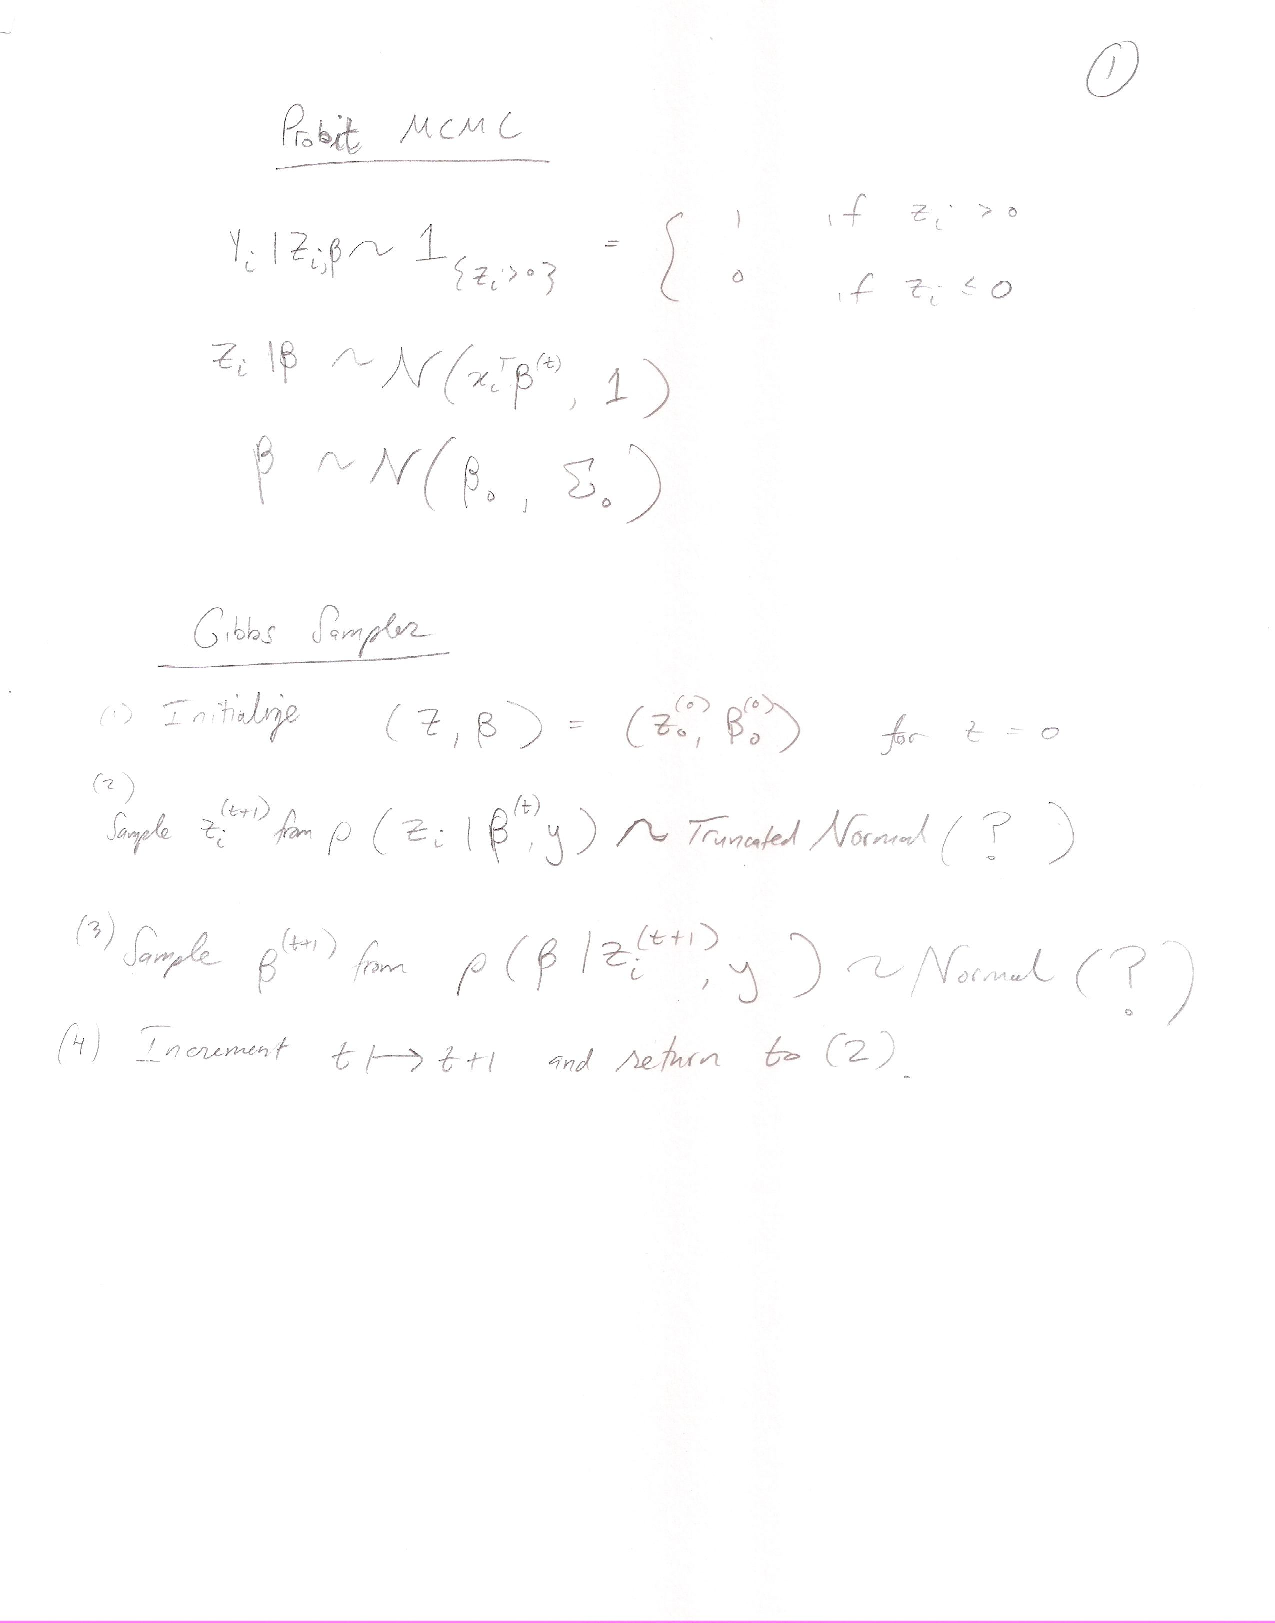
\includepdf[pages=1-5]{../gibbs_full_conditional_derivation.pdf}

\subsection{Verifying estimates on $\beta$}


We noticed that the standard errors for the mini data chunk are quite large. Table 1 shows that the posterior distribution for  $\beta_i, i = 1, \dots, 8$ almost covers the true beta in every case. Var1 and var5 are not exactly covered. The burn in time was very long ( $5 \times 10^5$) to get pretty good trace plots. Although var3 did struggle to fully converge. The trace plots and posterior density are not shown here. 
% latex table generated in R 3.0.1 by xtable 1.7-1 package
% Mon Dec  9 06:48:34 2013
\begin{table}[ht]
\caption{Estimates for $\hat{\beta}$ from the { \bf data chunk mini }}
\centering
\begin{tabular}{rrrrrrrrr}
  \hline
 & var1 & var2 & var3 & var4 & var5 & var6 & var7 & var8 \\ 
  \hline
post.  $\hat{\beta}$ 1\% & 0.655 & -0.188 & -9.216 & -0.636 & 1.112 & -0.528 & 0.866 & -1.107 \\ 
post.  $\hat{\beta}$ 99\% & 2.807 & 1.241 & -2.908 & 0.551 & 3.809 & 0.415 & 3.410 & 0.435 \\ 
  post. mean $\hat{\beta}$ & 1.564 & 0.482 & -5.295 & -0.029 & 2.179 & -0.044 & 1.936 & -0.291 \\ 
  true $\beta$& 0.568 & -0.106 & -2.059 & 0.121 & 1.053 & -0.102 & 1.233 & -0.027 \\ 
   \hline
\end{tabular}
\end{table}

{ \bf For data chunk 01, the posterior density covers $\beta$ in every case } with a $burnin = 8 \times 10^4$ and $niter  =  1 \times 20^4$.  The reason why $niter$ was so low was to be able to show a trace plot with a small enough file size, but even that produced too large of a file and so it was excluded. The trace plots were not convincing of convergence in several cases and if more time was allowed, we would have run the MCMC longer. 

% latex table generated in R 3.0.1 by xtable 1.7-1 package
% Mon Dec  9 07:15:28 2013
\begin{table}[ht]
\caption{Estimates for $\hat{\beta}$ from the {\bf data chunk 01 } show that $\beta$ is covered by the posterior in every case.}
\centering
\begin{tabular}{rrrrrrrrr}
  \hline
 & var1 & var2 & var3 & var4 & var5 & var6 & var7 & var8 \\ 
  \hline
post.  $\hat{\beta}$ 1\% & -0.002 & -1.243 & 0.180 & 1.788 & 1.396 & -1.268 & 2.080 & 0.649 \\ 
  post.  $\hat{\beta}$ 99\% & 0.363 & -0.776 & 0.549 & 2.554 & 2.044 & -0.791 & 2.927 & 1.092 \\ 
  post.  mean $\hat{\beta}$ & 0.183 & -1.000 & 0.362 & 2.159 & 1.708 & -1.018 & 2.488 & 0.858 \\ 
  true.beta & 0.140 & -0.973 & 0.308 & 1.868 & 1.486 & -0.948 & 2.416 & 0.803 \\ 
   \hline
\end{tabular}
\end{table}

\newpage 

\subsection{MCMC performance as the data size scales up.}

We were able finish running the code on all data chunks (01-04) but not the last (05). We ran the largest data chunk for over 16 hours but it did not even finish for the CPU. We started the GPU on data chunk 05, but it was terminated due to lack of time and because we know did not sample any faster on the order of $10^7$---the size of data chunk 05---in the comparative performance of question 1 (e) above. A small caveat is that the $maxtries$ argument is only 25 instead of 2000 for the Rcpp code. In the future, I would like to have kept them equal, but I forgot to change it and now it is too late. 

\begin{figure}[htbp] %  figure placement: here, top, bottom, or page
   \centering
   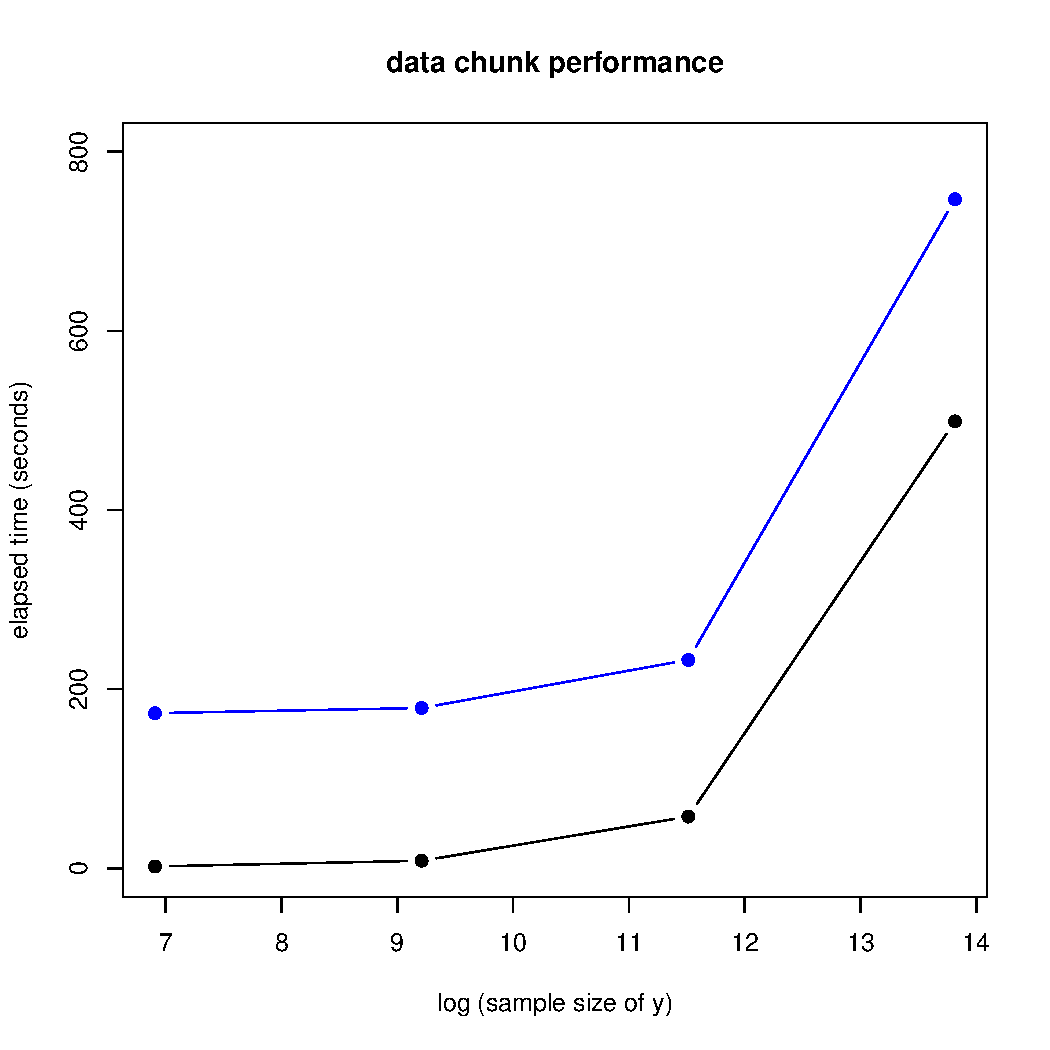
\includegraphics[width=4in]{../data_chunk_performance.pdf} 
   \caption{Probit MCMC comparative performance of CPU (black), GPU (blue). }
   \label{fig:mcmc_profile}
\end{figure}

What is interesting about Figure \ref{fig:mcmc_profile} is that the performance between the two hardware configurations seem to differ by a constant in the Probit MCMC case. This is likely the cost of copying the result from the device back to the host, but we did not confirm this suspicion.  We speculate that the GPU code would begin to outperform the CPU in the Probit MCMC example when the number of truncated normal samples is on the order of $10^8$ and above. This conjecture is based on the first performance evaluation of question 1. 

\section{Appendix A: Truncated Normal Sampler Code}

\subsection{GPU Kernel}
%%%%%%%% Insert  code %%%%%%%%%%%%%%%%%%%
\prettycode{gpu kernel}{../rtruncnorm.cu}
\subsection{CPU Truncated Normal Sampler}
This is virtually the same code as the GPU kernel, but written in Rcpp.
%%%%%%%% Insert  code %%%%%%%%%%%%%%%%%%%
\prettycode{cpu}{../rtruncnorm_cpu.cpp}



\section{Appendix B: Validate Sampler}
\subsection{Validate samplers}
\prettycode{}{../verify_rtruncnorm.r}


\section{Appendix C: Probit MCMC Code}
\subsection{Probit MCMC}
\prettycode{}{../probit_mcmc.r}


\end{document}  